% Created by tikzDevice version 0.6.1 on 2016-04-19 18:32:43
% !TEX encoding = UTF-8 Unicode
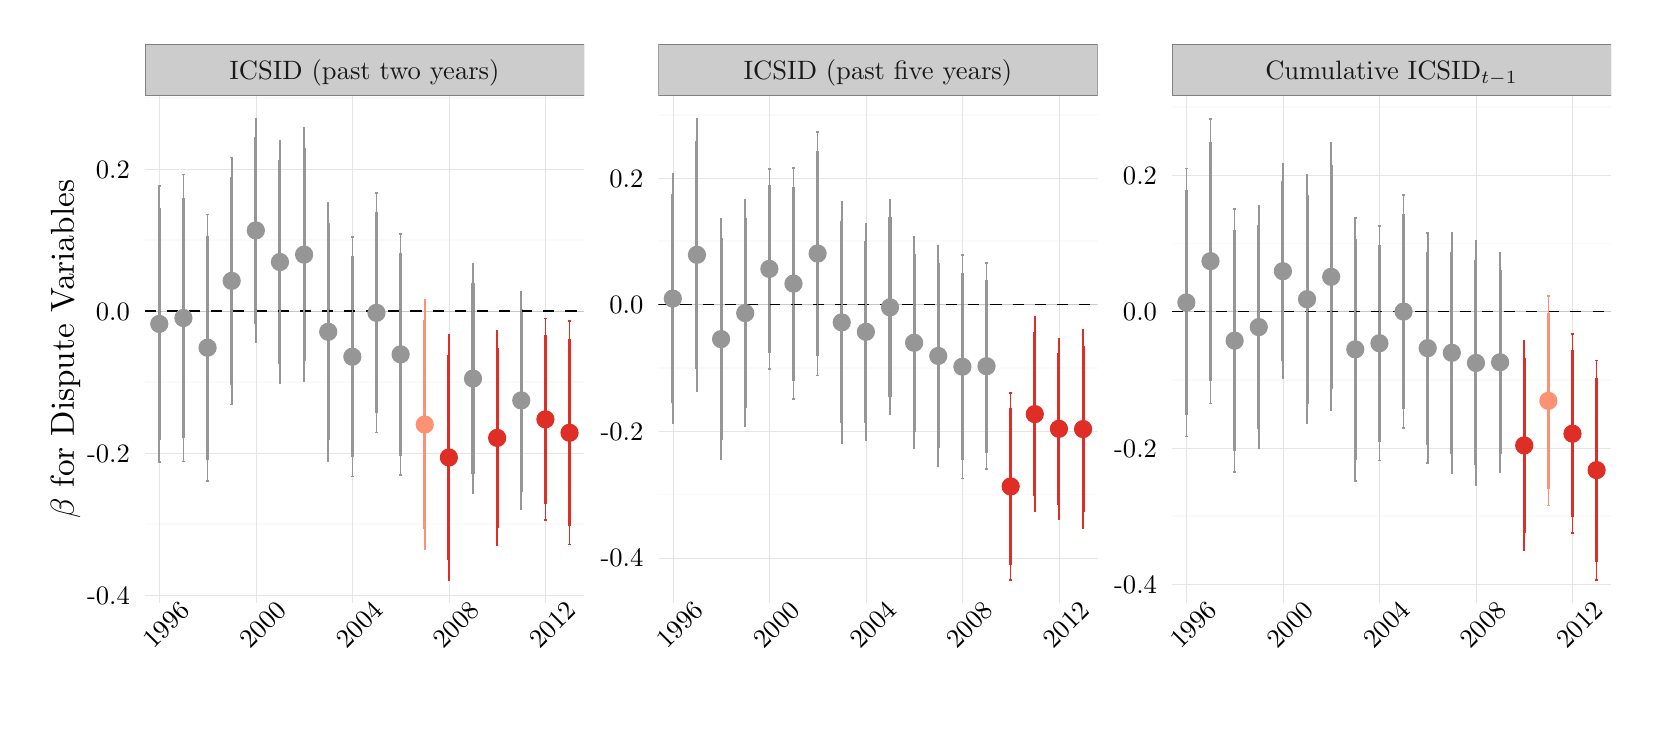
\begin{tikzpicture}[x=1pt,y=1pt]
\definecolor[named]{drawColor}{rgb}{0.00,0.00,0.00}
\definecolor[named]{fillColor}{rgb}{1.00,1.00,1.00}
\fill[color=fillColor,] (0,0) rectangle (578.16,252.94);
\begin{scope}
\path[clip] (  0.00,  0.00) rectangle (578.16,252.94);
\end{scope}
\begin{scope}
\path[clip] (  0.00,  0.00) rectangle (578.16,252.94);
\end{scope}
\begin{scope}
\path[clip] (  0.00,  0.00) rectangle (578.16,252.94);
\end{scope}
\begin{scope}
\path[clip] (  0.00,  0.00) rectangle (578.16,252.94);
\end{scope}
\begin{scope}
\path[clip] (  0.00,  0.00) rectangle (578.16,252.94);
\end{scope}
\begin{scope}
\path[clip] (  0.00,  0.00) rectangle (578.16,252.94);
\end{scope}
\begin{scope}
\path[clip] (  0.00,  0.00) rectangle (578.16,252.94);
\end{scope}
\begin{scope}
\path[clip] (  0.00,  0.00) rectangle (578.16,252.94);
\end{scope}
\begin{scope}
\path[clip] (  0.00,  0.00) rectangle (578.16,252.94);
\end{scope}
\begin{scope}
\path[clip] (  0.00,  0.00) rectangle (578.16,252.94);
\end{scope}
\begin{scope}
\path[clip] (  0.00,  0.00) rectangle (578.16,252.94);
\end{scope}
\begin{scope}
\path[clip] (  0.00,  0.00) rectangle (578.16,252.94);
\end{scope}
\begin{scope}
\path[clip] (  0.00,  0.00) rectangle (578.16,252.94);
\end{scope}
\begin{scope}
\path[clip] (  0.00,  0.00) rectangle (578.16,252.94);
\end{scope}
\begin{scope}
\path[clip] (  0.00,  0.00) rectangle (578.16,252.94);
\end{scope}
\begin{scope}
\path[clip] (  0.00,  0.00) rectangle (578.16,252.94);
\end{scope}
\begin{scope}
\path[clip] (  0.00,  0.00) rectangle (578.16,252.94);
\end{scope}
\begin{scope}
\path[clip] (  0.00,  0.00) rectangle (578.16,252.94);
\end{scope}
\begin{scope}
\path[clip] (  0.00,  0.00) rectangle (578.16,252.94);
\definecolor[named]{drawColor}{rgb}{1.00,1.00,1.00}
\definecolor[named]{fillColor}{rgb}{1.00,1.00,1.00}

\draw[color=drawColor,line width= 0.6pt,line cap=round,line join=round,fill=fillColor,] ( -0.00,  0.00) rectangle (578.16,252.94);
\end{scope}
\begin{scope}
\path[clip] (  0.00,  0.00) rectangle (578.16,252.94);
\end{scope}
\begin{scope}
\path[clip] ( 42.33, 45.11) rectangle (201.03,228.33);
\definecolor[named]{fillColor}{rgb}{1.00,1.00,1.00}

\draw[fill=fillColor,draw opacity=0.00,] ( 42.33, 45.11) rectangle (201.03,228.33);
\definecolor[named]{drawColor}{rgb}{0.98,0.98,0.98}

\draw[color=drawColor,line width= 0.6pt,line join=round,fill opacity=0.00,] ( 42.33, 73.50) --
	(201.03, 73.50);

\draw[color=drawColor,line width= 0.6pt,line join=round,fill opacity=0.00,] ( 42.33,124.81) --
	(201.03,124.81);

\draw[color=drawColor,line width= 0.6pt,line join=round,fill opacity=0.00,] ( 42.33,176.13) --
	(201.03,176.13);

\draw[color=drawColor,line width= 0.6pt,line join=round,fill opacity=0.00,] ( 42.33,227.44) --
	(201.03,227.44);
\definecolor[named]{drawColor}{rgb}{0.90,0.90,0.90}

\draw[color=drawColor,line width= 0.2pt,line join=round,fill opacity=0.00,] ( 42.33, 47.84) --
	(201.03, 47.84);

\draw[color=drawColor,line width= 0.2pt,line join=round,fill opacity=0.00,] ( 42.33, 99.15) --
	(201.03, 99.15);

\draw[color=drawColor,line width= 0.2pt,line join=round,fill opacity=0.00,] ( 42.33,150.47) --
	(201.03,150.47);

\draw[color=drawColor,line width= 0.2pt,line join=round,fill opacity=0.00,] ( 42.33,201.78) --
	(201.03,201.78);

\draw[color=drawColor,line width= 0.2pt,line join=round,fill opacity=0.00,] ( 47.56, 45.11) --
	( 47.56,228.33);

\draw[color=drawColor,line width= 0.2pt,line join=round,fill opacity=0.00,] ( 82.44, 45.11) --
	( 82.44,228.33);

\draw[color=drawColor,line width= 0.2pt,line join=round,fill opacity=0.00,] (117.32, 45.11) --
	(117.32,228.33);

\draw[color=drawColor,line width= 0.2pt,line join=round,fill opacity=0.00,] (152.20, 45.11) --
	(152.20,228.33);

\draw[color=drawColor,line width= 0.2pt,line join=round,fill opacity=0.00,] (187.08, 45.11) --
	(187.08,228.33);
\definecolor[named]{drawColor}{rgb}{0.59,0.59,0.59}
\definecolor[named]{fillColor}{rgb}{0.59,0.59,0.59}

\draw[color=drawColor,line width= 0.3pt,line join=round,fill=fillColor,fill opacity=0.30,draw opacity=0.30,] ( 47.56, 96.06) -- ( 47.56,195.73);

\draw[color=drawColor,line width= 0.3pt,line join=round,fill=fillColor,fill opacity=0.30,draw opacity=0.30,] ( 56.28, 96.18) -- ( 56.28,199.86);

\draw[color=drawColor,line width= 0.3pt,line join=round,fill=fillColor,fill opacity=0.30,draw opacity=0.30,] ( 65.00, 89.13) -- ( 65.00,185.46);

\draw[color=drawColor,line width= 0.3pt,line join=round,fill=fillColor,fill opacity=0.30,draw opacity=0.30,] ( 73.72,116.81) -- ( 73.72,206.08);

\draw[color=drawColor,line width= 0.3pt,line join=round,fill=fillColor,fill opacity=0.30,draw opacity=0.30,] ( 82.44,139.36) -- ( 82.44,220.01);

\draw[color=drawColor,line width= 0.3pt,line join=round,fill=fillColor,fill opacity=0.30,draw opacity=0.30,] ( 91.16,124.31) -- ( 91.16,212.21);

\draw[color=drawColor,line width= 0.3pt,line join=round,fill=fillColor,fill opacity=0.30,draw opacity=0.30,] ( 99.88,125.06) -- ( 99.88,216.79);

\draw[color=drawColor,line width= 0.3pt,line join=round,fill=fillColor,fill opacity=0.30,draw opacity=0.30,] (108.60, 96.32) -- (108.60,189.76);

\draw[color=drawColor,line width= 0.3pt,line join=round,fill=fillColor,fill opacity=0.30,draw opacity=0.30,] (117.32, 90.80) -- (117.32,177.26);

\draw[color=drawColor,line width= 0.3pt,line join=round,fill=fillColor,fill opacity=0.30,draw opacity=0.30,] (126.04,106.67) -- (126.04,193.12);

\draw[color=drawColor,line width= 0.3pt,line join=round,fill=fillColor,fill opacity=0.30,draw opacity=0.30,] (134.76, 91.27) -- (134.76,178.50);
\definecolor[named]{drawColor}{rgb}{0.99,0.57,0.45}
\definecolor[named]{fillColor}{rgb}{0.99,0.57,0.45}

\draw[color=drawColor,line width= 0.3pt,line join=round,fill=fillColor,fill opacity=0.30,draw opacity=0.30,] (143.48, 64.36) -- (143.48,154.69);
\definecolor[named]{drawColor}{rgb}{0.87,0.18,0.15}
\definecolor[named]{fillColor}{rgb}{0.87,0.18,0.15}

\draw[color=drawColor,line width= 0.3pt,line join=round,fill=fillColor,fill opacity=0.30,draw opacity=0.30,] (152.20, 53.44) -- (152.20,141.81);
\definecolor[named]{drawColor}{rgb}{0.59,0.59,0.59}
\definecolor[named]{fillColor}{rgb}{0.59,0.59,0.59}

\draw[color=drawColor,line width= 0.3pt,line join=round,fill=fillColor,fill opacity=0.30,draw opacity=0.30,] (160.92, 84.84) -- (160.92,167.44);
\definecolor[named]{drawColor}{rgb}{0.87,0.18,0.15}
\definecolor[named]{fillColor}{rgb}{0.87,0.18,0.15}

\draw[color=drawColor,line width= 0.3pt,line join=round,fill=fillColor,fill opacity=0.30,draw opacity=0.30,] (169.64, 65.95) -- (169.64,143.45);
\definecolor[named]{drawColor}{rgb}{0.59,0.59,0.59}
\definecolor[named]{fillColor}{rgb}{0.59,0.59,0.59}

\draw[color=drawColor,line width= 0.3pt,line join=round,fill=fillColor,fill opacity=0.30,draw opacity=0.30,] (178.36, 78.96) -- (178.36,157.52);
\definecolor[named]{drawColor}{rgb}{0.87,0.18,0.15}
\definecolor[named]{fillColor}{rgb}{0.87,0.18,0.15}

\draw[color=drawColor,line width= 0.3pt,line join=round,fill=fillColor,fill opacity=0.30,draw opacity=0.30,] (187.08, 74.93) -- (187.08,147.88);

\draw[color=drawColor,line width= 0.3pt,line join=round,fill=fillColor,fill opacity=0.30,draw opacity=0.30,] (195.80, 66.20) -- (195.80,146.91);
\definecolor[named]{drawColor}{rgb}{0.59,0.59,0.59}
\definecolor[named]{fillColor}{rgb}{0.59,0.59,0.59}

\draw[color=drawColor,line width= 1.1pt,line join=round,fill=fillColor,] ( 47.56,104.07) -- ( 47.56,187.72);

\draw[color=drawColor,line width= 1.1pt,line join=round,fill=fillColor,] ( 56.28,104.51) -- ( 56.28,191.52);

\draw[color=drawColor,line width= 1.1pt,line join=round,fill=fillColor,] ( 65.00, 96.88) -- ( 65.00,177.71);

\draw[color=drawColor,line width= 1.1pt,line join=round,fill=fillColor,] ( 73.72,123.99) -- ( 73.72,198.91);

\draw[color=drawColor,line width= 1.1pt,line join=round,fill=fillColor,] ( 82.44,145.84) -- ( 82.44,213.52);

\draw[color=drawColor,line width= 1.1pt,line join=round,fill=fillColor,] ( 91.16,131.38) -- ( 91.16,205.14);

\draw[color=drawColor,line width= 1.1pt,line join=round,fill=fillColor,] ( 99.88,132.44) -- ( 99.88,209.42);

\draw[color=drawColor,line width= 1.1pt,line join=round,fill=fillColor,] (108.60,103.83) -- (108.60,182.25);

\draw[color=drawColor,line width= 1.1pt,line join=round,fill=fillColor,] (117.32, 97.75) -- (117.32,170.31);

\draw[color=drawColor,line width= 1.1pt,line join=round,fill=fillColor,] (126.04,113.62) -- (126.04,186.17);

\draw[color=drawColor,line width= 1.1pt,line join=round,fill=fillColor,] (134.76, 98.28) -- (134.76,171.49);
\definecolor[named]{drawColor}{rgb}{0.99,0.57,0.45}
\definecolor[named]{fillColor}{rgb}{0.99,0.57,0.45}

\draw[color=drawColor,line width= 1.1pt,line join=round,fill=fillColor,] (143.48, 71.62) -- (143.48,147.43);
\definecolor[named]{drawColor}{rgb}{0.87,0.18,0.15}
\definecolor[named]{fillColor}{rgb}{0.87,0.18,0.15}

\draw[color=drawColor,line width= 1.1pt,line join=round,fill=fillColor,] (152.20, 60.55) -- (152.20,134.71);
\definecolor[named]{drawColor}{rgb}{0.59,0.59,0.59}
\definecolor[named]{fillColor}{rgb}{0.59,0.59,0.59}

\draw[color=drawColor,line width= 1.1pt,line join=round,fill=fillColor,] (160.92, 91.48) -- (160.92,160.80);
\definecolor[named]{drawColor}{rgb}{0.87,0.18,0.15}
\definecolor[named]{fillColor}{rgb}{0.87,0.18,0.15}

\draw[color=drawColor,line width= 1.1pt,line join=round,fill=fillColor,] (169.64, 72.18) -- (169.64,137.22);
\definecolor[named]{drawColor}{rgb}{0.59,0.59,0.59}
\definecolor[named]{fillColor}{rgb}{0.59,0.59,0.59}

\draw[color=drawColor,line width= 1.1pt,line join=round,fill=fillColor,] (178.36, 85.28) -- (178.36,151.20);
\definecolor[named]{drawColor}{rgb}{0.87,0.18,0.15}
\definecolor[named]{fillColor}{rgb}{0.87,0.18,0.15}

\draw[color=drawColor,line width= 1.1pt,line join=round,fill=fillColor,] (187.08, 80.80) -- (187.08,142.02);

\draw[color=drawColor,line width= 1.1pt,line join=round,fill=fillColor,] (195.80, 72.69) -- (195.80,140.42);
\definecolor[named]{drawColor}{rgb}{0.00,0.00,0.00}
\definecolor[named]{fillColor}{rgb}{0.00,0.00,0.00}

\draw[color=drawColor,line width= 0.6pt,dash pattern=on 4pt off 4pt ,line join=round,fill=fillColor,] ( 42.33,150.47) -- (201.03,150.47);
\definecolor[named]{drawColor}{rgb}{0.59,0.59,0.59}
\definecolor[named]{fillColor}{rgb}{0.59,0.59,0.59}

\draw[color=drawColor,line width= 0.4pt,line cap=round,line join=round,fill=fillColor,] ( 47.56,145.89) circle (  3.09);

\draw[color=drawColor,line width= 0.4pt,line cap=round,line join=round,fill=fillColor,] ( 56.28,148.02) circle (  3.09);

\draw[color=drawColor,line width= 0.4pt,line cap=round,line join=round,fill=fillColor,] ( 65.00,137.29) circle (  3.09);

\draw[color=drawColor,line width= 0.4pt,line cap=round,line join=round,fill=fillColor,] ( 73.72,161.45) circle (  3.09);

\draw[color=drawColor,line width= 0.4pt,line cap=round,line join=round,fill=fillColor,] ( 82.44,179.68) circle (  3.09);

\draw[color=drawColor,line width= 0.4pt,line cap=round,line join=round,fill=fillColor,] ( 91.16,168.26) circle (  3.09);

\draw[color=drawColor,line width= 0.4pt,line cap=round,line join=round,fill=fillColor,] ( 99.88,170.93) circle (  3.09);

\draw[color=drawColor,line width= 0.4pt,line cap=round,line join=round,fill=fillColor,] (108.60,143.04) circle (  3.09);

\draw[color=drawColor,line width= 0.4pt,line cap=round,line join=round,fill=fillColor,] (117.32,134.03) circle (  3.09);

\draw[color=drawColor,line width= 0.4pt,line cap=round,line join=round,fill=fillColor,] (126.04,149.90) circle (  3.09);

\draw[color=drawColor,line width= 0.4pt,line cap=round,line join=round,fill=fillColor,] (134.76,134.89) circle (  3.09);
\definecolor[named]{drawColor}{rgb}{0.99,0.57,0.45}
\definecolor[named]{fillColor}{rgb}{0.99,0.57,0.45}

\draw[color=drawColor,line width= 0.4pt,line cap=round,line join=round,fill=fillColor,] (143.48,109.52) circle (  3.09);
\definecolor[named]{drawColor}{rgb}{0.87,0.18,0.15}
\definecolor[named]{fillColor}{rgb}{0.87,0.18,0.15}

\draw[color=drawColor,line width= 0.4pt,line cap=round,line join=round,fill=fillColor,] (152.20, 97.63) circle (  3.09);
\definecolor[named]{drawColor}{rgb}{0.59,0.59,0.59}
\definecolor[named]{fillColor}{rgb}{0.59,0.59,0.59}

\draw[color=drawColor,line width= 0.4pt,line cap=round,line join=round,fill=fillColor,] (160.92,126.14) circle (  3.09);
\definecolor[named]{drawColor}{rgb}{0.87,0.18,0.15}
\definecolor[named]{fillColor}{rgb}{0.87,0.18,0.15}

\draw[color=drawColor,line width= 0.4pt,line cap=round,line join=round,fill=fillColor,] (169.64,104.70) circle (  3.09);
\definecolor[named]{drawColor}{rgb}{0.59,0.59,0.59}
\definecolor[named]{fillColor}{rgb}{0.59,0.59,0.59}

\draw[color=drawColor,line width= 0.4pt,line cap=round,line join=round,fill=fillColor,] (178.36,118.24) circle (  3.09);
\definecolor[named]{drawColor}{rgb}{0.87,0.18,0.15}
\definecolor[named]{fillColor}{rgb}{0.87,0.18,0.15}

\draw[color=drawColor,line width= 0.4pt,line cap=round,line join=round,fill=fillColor,] (187.08,111.41) circle (  3.09);

\draw[color=drawColor,line width= 0.4pt,line cap=round,line join=round,fill=fillColor,] (195.80,106.55) circle (  3.09);
\definecolor[named]{drawColor}{rgb}{0.59,0.59,0.59}
\definecolor[named]{fillColor}{rgb}{0.59,0.59,0.59}

\draw[color=drawColor,line width= 0.6pt,line join=round,] ( 47.12,195.73) --
	( 48.00,195.73);

\draw[color=drawColor,line width= 0.6pt,line join=round,] ( 47.56,195.73) --
	( 47.56, 96.06);

\draw[color=drawColor,line width= 0.6pt,line join=round,] ( 47.12, 96.06) --
	( 48.00, 96.06);

\draw[color=drawColor,line width= 0.6pt,line join=round,] ( 55.84,199.86) --
	( 56.72,199.86);

\draw[color=drawColor,line width= 0.6pt,line join=round,] ( 56.28,199.86) --
	( 56.28, 96.18);

\draw[color=drawColor,line width= 0.6pt,line join=round,] ( 55.84, 96.18) --
	( 56.72, 96.18);

\draw[color=drawColor,line width= 0.6pt,line join=round,] ( 64.56,185.46) --
	( 65.44,185.46);

\draw[color=drawColor,line width= 0.6pt,line join=round,] ( 65.00,185.46) --
	( 65.00, 89.13);

\draw[color=drawColor,line width= 0.6pt,line join=round,] ( 64.56, 89.13) --
	( 65.44, 89.13);

\draw[color=drawColor,line width= 0.6pt,line join=round,] ( 73.28,206.08) --
	( 74.16,206.08);

\draw[color=drawColor,line width= 0.6pt,line join=round,] ( 73.72,206.08) --
	( 73.72,116.81);

\draw[color=drawColor,line width= 0.6pt,line join=round,] ( 73.28,116.81) --
	( 74.16,116.81);

\draw[color=drawColor,line width= 0.6pt,line join=round,] ( 82.00,220.01) --
	( 82.88,220.01);

\draw[color=drawColor,line width= 0.6pt,line join=round,] ( 82.44,220.01) --
	( 82.44,139.36);

\draw[color=drawColor,line width= 0.6pt,line join=round,] ( 82.00,139.36) --
	( 82.88,139.36);

\draw[color=drawColor,line width= 0.6pt,line join=round,] ( 90.72,212.21) --
	( 91.60,212.21);

\draw[color=drawColor,line width= 0.6pt,line join=round,] ( 91.16,212.21) --
	( 91.16,124.31);

\draw[color=drawColor,line width= 0.6pt,line join=round,] ( 90.72,124.31) --
	( 91.60,124.31);

\draw[color=drawColor,line width= 0.6pt,line join=round,] ( 99.44,216.79) --
	(100.31,216.79);

\draw[color=drawColor,line width= 0.6pt,line join=round,] ( 99.88,216.79) --
	( 99.88,125.06);

\draw[color=drawColor,line width= 0.6pt,line join=round,] ( 99.44,125.06) --
	(100.31,125.06);

\draw[color=drawColor,line width= 0.6pt,line join=round,] (108.16,189.76) --
	(109.03,189.76);

\draw[color=drawColor,line width= 0.6pt,line join=round,] (108.60,189.76) --
	(108.60, 96.32);

\draw[color=drawColor,line width= 0.6pt,line join=round,] (108.16, 96.32) --
	(109.03, 96.32);

\draw[color=drawColor,line width= 0.6pt,line join=round,] (116.88,177.26) --
	(117.75,177.26);

\draw[color=drawColor,line width= 0.6pt,line join=round,] (117.32,177.26) --
	(117.32, 90.80);

\draw[color=drawColor,line width= 0.6pt,line join=round,] (116.88, 90.80) --
	(117.75, 90.80);

\draw[color=drawColor,line width= 0.6pt,line join=round,] (125.60,193.12) --
	(126.47,193.12);

\draw[color=drawColor,line width= 0.6pt,line join=round,] (126.04,193.12) --
	(126.04,106.67);

\draw[color=drawColor,line width= 0.6pt,line join=round,] (125.60,106.67) --
	(126.47,106.67);

\draw[color=drawColor,line width= 0.6pt,line join=round,] (134.32,178.50) --
	(135.19,178.50);

\draw[color=drawColor,line width= 0.6pt,line join=round,] (134.76,178.50) --
	(134.76, 91.27);

\draw[color=drawColor,line width= 0.6pt,line join=round,] (134.32, 91.27) --
	(135.19, 91.27);
\definecolor[named]{drawColor}{rgb}{0.99,0.57,0.45}
\definecolor[named]{fillColor}{rgb}{0.99,0.57,0.45}

\draw[color=drawColor,line width= 0.6pt,line join=round,] (143.04,154.69) --
	(143.91,154.69);

\draw[color=drawColor,line width= 0.6pt,line join=round,] (143.48,154.69) --
	(143.48, 64.36);

\draw[color=drawColor,line width= 0.6pt,line join=round,] (143.04, 64.36) --
	(143.91, 64.36);
\definecolor[named]{drawColor}{rgb}{0.87,0.18,0.15}
\definecolor[named]{fillColor}{rgb}{0.87,0.18,0.15}

\draw[color=drawColor,line width= 0.6pt,line join=round,] (151.76,141.81) --
	(152.63,141.81);

\draw[color=drawColor,line width= 0.6pt,line join=round,] (152.20,141.81) --
	(152.20, 53.44);

\draw[color=drawColor,line width= 0.6pt,line join=round,] (151.76, 53.44) --
	(152.63, 53.44);
\definecolor[named]{drawColor}{rgb}{0.59,0.59,0.59}
\definecolor[named]{fillColor}{rgb}{0.59,0.59,0.59}

\draw[color=drawColor,line width= 0.6pt,line join=round,] (160.48,167.44) --
	(161.35,167.44);

\draw[color=drawColor,line width= 0.6pt,line join=round,] (160.92,167.44) --
	(160.92, 84.84);

\draw[color=drawColor,line width= 0.6pt,line join=round,] (160.48, 84.84) --
	(161.35, 84.84);
\definecolor[named]{drawColor}{rgb}{0.87,0.18,0.15}
\definecolor[named]{fillColor}{rgb}{0.87,0.18,0.15}

\draw[color=drawColor,line width= 0.6pt,line join=round,] (169.20,143.45) --
	(170.07,143.45);

\draw[color=drawColor,line width= 0.6pt,line join=round,] (169.64,143.45) --
	(169.64, 65.95);

\draw[color=drawColor,line width= 0.6pt,line join=round,] (169.20, 65.95) --
	(170.07, 65.95);
\definecolor[named]{drawColor}{rgb}{0.59,0.59,0.59}
\definecolor[named]{fillColor}{rgb}{0.59,0.59,0.59}

\draw[color=drawColor,line width= 0.6pt,line join=round,] (177.92,157.52) --
	(178.79,157.52);

\draw[color=drawColor,line width= 0.6pt,line join=round,] (178.36,157.52) --
	(178.36, 78.96);

\draw[color=drawColor,line width= 0.6pt,line join=round,] (177.92, 78.96) --
	(178.79, 78.96);
\definecolor[named]{drawColor}{rgb}{0.87,0.18,0.15}
\definecolor[named]{fillColor}{rgb}{0.87,0.18,0.15}

\draw[color=drawColor,line width= 0.6pt,line join=round,] (186.64,147.88) --
	(187.51,147.88);

\draw[color=drawColor,line width= 0.6pt,line join=round,] (187.08,147.88) --
	(187.08, 74.93);

\draw[color=drawColor,line width= 0.6pt,line join=round,] (186.64, 74.93) --
	(187.51, 74.93);

\draw[color=drawColor,line width= 0.6pt,line join=round,] (195.36,146.91) --
	(196.23,146.91);

\draw[color=drawColor,line width= 0.6pt,line join=round,] (195.80,146.91) --
	(195.80, 66.20);

\draw[color=drawColor,line width= 0.6pt,line join=round,] (195.36, 66.20) --
	(196.23, 66.20);
\end{scope}
\begin{scope}
\path[clip] (  0.00,  0.00) rectangle (578.16,252.94);
\end{scope}
\begin{scope}
\path[clip] (227.89, 45.11) rectangle (386.59,228.33);
\definecolor[named]{fillColor}{rgb}{1.00,1.00,1.00}

\draw[fill=fillColor,draw opacity=0.00,] (227.89, 45.11) rectangle (386.59,228.33);
\definecolor[named]{drawColor}{rgb}{0.98,0.98,0.98}

\draw[color=drawColor,line width= 0.6pt,line join=round,fill opacity=0.00,] (227.89, 84.26) --
	(386.59, 84.26);

\draw[color=drawColor,line width= 0.6pt,line join=round,fill opacity=0.00,] (227.89,130.00) --
	(386.59,130.00);

\draw[color=drawColor,line width= 0.6pt,line join=round,fill opacity=0.00,] (227.89,175.75) --
	(386.59,175.75);

\draw[color=drawColor,line width= 0.6pt,line join=round,fill opacity=0.00,] (227.89,221.49) --
	(386.59,221.49);
\definecolor[named]{drawColor}{rgb}{0.90,0.90,0.90}

\draw[color=drawColor,line width= 0.2pt,line join=round,fill opacity=0.00,] (227.89, 61.38) --
	(386.59, 61.38);

\draw[color=drawColor,line width= 0.2pt,line join=round,fill opacity=0.00,] (227.89,107.13) --
	(386.59,107.13);

\draw[color=drawColor,line width= 0.2pt,line join=round,fill opacity=0.00,] (227.89,152.87) --
	(386.59,152.87);

\draw[color=drawColor,line width= 0.2pt,line join=round,fill opacity=0.00,] (227.89,198.62) --
	(386.59,198.62);

\draw[color=drawColor,line width= 0.2pt,line join=round,fill opacity=0.00,] (233.12, 45.11) --
	(233.12,228.33);

\draw[color=drawColor,line width= 0.2pt,line join=round,fill opacity=0.00,] (268.00, 45.11) --
	(268.00,228.33);

\draw[color=drawColor,line width= 0.2pt,line join=round,fill opacity=0.00,] (302.88, 45.11) --
	(302.88,228.33);

\draw[color=drawColor,line width= 0.2pt,line join=round,fill opacity=0.00,] (337.76, 45.11) --
	(337.76,228.33);

\draw[color=drawColor,line width= 0.2pt,line join=round,fill opacity=0.00,] (372.64, 45.11) --
	(372.64,228.33);
\definecolor[named]{drawColor}{rgb}{0.59,0.59,0.59}
\definecolor[named]{fillColor}{rgb}{0.59,0.59,0.59}

\draw[color=drawColor,line width= 0.3pt,line join=round,fill=fillColor,fill opacity=0.30,draw opacity=0.30,] (233.12,109.97) -- (233.12,200.12);

\draw[color=drawColor,line width= 0.3pt,line join=round,fill=fillColor,fill opacity=0.30,draw opacity=0.30,] (241.84,121.71) -- (241.84,220.01);

\draw[color=drawColor,line width= 0.3pt,line join=round,fill=fillColor,fill opacity=0.30,draw opacity=0.30,] (250.56, 96.93) -- (250.56,183.88);

\draw[color=drawColor,line width= 0.3pt,line join=round,fill=fillColor,fill opacity=0.30,draw opacity=0.30,] (259.28,108.99) -- (259.28,190.62);

\draw[color=drawColor,line width= 0.3pt,line join=round,fill=fillColor,fill opacity=0.30,draw opacity=0.30,] (268.00,129.62) -- (268.00,201.92);

\draw[color=drawColor,line width= 0.3pt,line join=round,fill=fillColor,fill opacity=0.30,draw opacity=0.30,] (276.72,118.73) -- (276.72,202.16);

\draw[color=drawColor,line width= 0.3pt,line join=round,fill=fillColor,fill opacity=0.30,draw opacity=0.30,] (285.44,127.30) -- (285.44,215.35);

\draw[color=drawColor,line width= 0.3pt,line join=round,fill=fillColor,fill opacity=0.30,draw opacity=0.30,] (294.16,102.93) -- (294.16,189.95);

\draw[color=drawColor,line width= 0.3pt,line join=round,fill=fillColor,fill opacity=0.30,draw opacity=0.30,] (302.88,103.98) -- (302.88,182.08);

\draw[color=drawColor,line width= 0.3pt,line join=round,fill=fillColor,fill opacity=0.30,draw opacity=0.30,] (311.60,113.17) -- (311.60,190.58);

\draw[color=drawColor,line width= 0.3pt,line join=round,fill=fillColor,fill opacity=0.30,draw opacity=0.30,] (320.32,100.85) -- (320.32,177.30);

\draw[color=drawColor,line width= 0.3pt,line join=round,fill=fillColor,fill opacity=0.30,draw opacity=0.30,] (329.04, 94.51) -- (329.04,174.13);

\draw[color=drawColor,line width= 0.3pt,line join=round,fill=fillColor,fill opacity=0.30,draw opacity=0.30,] (337.76, 90.08) -- (337.76,170.78);

\draw[color=drawColor,line width= 0.3pt,line join=round,fill=fillColor,fill opacity=0.30,draw opacity=0.30,] (346.48, 93.42) -- (346.48,167.79);
\definecolor[named]{drawColor}{rgb}{0.87,0.18,0.15}
\definecolor[named]{fillColor}{rgb}{0.87,0.18,0.15}

\draw[color=drawColor,line width= 0.3pt,line join=round,fill=fillColor,fill opacity=0.30,draw opacity=0.30,] (355.20, 53.44) -- (355.20,120.86);

\draw[color=drawColor,line width= 0.3pt,line join=round,fill=fillColor,fill opacity=0.30,draw opacity=0.30,] (363.92, 78.07) -- (363.92,148.53);

\draw[color=drawColor,line width= 0.3pt,line join=round,fill=fillColor,fill opacity=0.30,draw opacity=0.30,] (372.64, 75.36) -- (372.64,140.63);

\draw[color=drawColor,line width= 0.3pt,line join=round,fill=fillColor,fill opacity=0.30,draw opacity=0.30,] (381.36, 72.13) -- (381.36,143.68);
\definecolor[named]{drawColor}{rgb}{0.59,0.59,0.59}
\definecolor[named]{fillColor}{rgb}{0.59,0.59,0.59}

\draw[color=drawColor,line width= 1.1pt,line join=round,fill=fillColor,] (233.12,117.22) -- (233.12,192.88);

\draw[color=drawColor,line width= 1.1pt,line join=round,fill=fillColor,] (241.84,129.61) -- (241.84,212.10);

\draw[color=drawColor,line width= 1.1pt,line join=round,fill=fillColor,] (250.56,103.92) -- (250.56,176.89);

\draw[color=drawColor,line width= 1.1pt,line join=round,fill=fillColor,] (259.28,115.55) -- (259.28,184.05);

\draw[color=drawColor,line width= 1.1pt,line join=round,fill=fillColor,] (268.00,135.44) -- (268.00,196.11);

\draw[color=drawColor,line width= 1.1pt,line join=round,fill=fillColor,] (276.72,125.43) -- (276.72,195.46);

\draw[color=drawColor,line width= 1.1pt,line join=round,fill=fillColor,] (285.44,134.38) -- (285.44,208.27);

\draw[color=drawColor,line width= 1.1pt,line join=round,fill=fillColor,] (294.16,109.93) -- (294.16,182.95);

\draw[color=drawColor,line width= 1.1pt,line join=round,fill=fillColor,] (302.88,110.26) -- (302.88,175.80);

\draw[color=drawColor,line width= 1.1pt,line join=round,fill=fillColor,] (311.60,119.39) -- (311.60,184.36);

\draw[color=drawColor,line width= 1.1pt,line join=round,fill=fillColor,] (320.32,107.00) -- (320.32,171.16);

\draw[color=drawColor,line width= 1.1pt,line join=round,fill=fillColor,] (329.04,100.91) -- (329.04,167.73);

\draw[color=drawColor,line width= 1.1pt,line join=round,fill=fillColor,] (337.76, 96.57) -- (337.76,164.29);

\draw[color=drawColor,line width= 1.1pt,line join=round,fill=fillColor,] (346.48, 99.40) -- (346.48,161.81);
\definecolor[named]{drawColor}{rgb}{0.87,0.18,0.15}
\definecolor[named]{fillColor}{rgb}{0.87,0.18,0.15}

\draw[color=drawColor,line width= 1.1pt,line join=round,fill=fillColor,] (355.20, 58.86) -- (355.20,115.44);

\draw[color=drawColor,line width= 1.1pt,line join=round,fill=fillColor,] (363.92, 83.74) -- (363.92,142.86);

\draw[color=drawColor,line width= 1.1pt,line join=round,fill=fillColor,] (372.64, 80.61) -- (372.64,135.38);

\draw[color=drawColor,line width= 1.1pt,line join=round,fill=fillColor,] (381.36, 77.88) -- (381.36,137.93);
\definecolor[named]{drawColor}{rgb}{0.00,0.00,0.00}
\definecolor[named]{fillColor}{rgb}{0.00,0.00,0.00}

\draw[color=drawColor,line width= 0.6pt,dash pattern=on 4pt off 4pt ,line join=round,fill=fillColor,] (227.89,152.87) -- (386.59,152.87);
\definecolor[named]{drawColor}{rgb}{0.59,0.59,0.59}
\definecolor[named]{fillColor}{rgb}{0.59,0.59,0.59}

\draw[color=drawColor,line width= 0.4pt,line cap=round,line join=round,fill=fillColor,] (233.12,155.05) circle (  3.09);

\draw[color=drawColor,line width= 0.4pt,line cap=round,line join=round,fill=fillColor,] (241.84,170.86) circle (  3.09);

\draw[color=drawColor,line width= 0.4pt,line cap=round,line join=round,fill=fillColor,] (250.56,140.40) circle (  3.09);

\draw[color=drawColor,line width= 0.4pt,line cap=round,line join=round,fill=fillColor,] (259.28,149.80) circle (  3.09);

\draw[color=drawColor,line width= 0.4pt,line cap=round,line join=round,fill=fillColor,] (268.00,165.77) circle (  3.09);

\draw[color=drawColor,line width= 0.4pt,line cap=round,line join=round,fill=fillColor,] (276.72,160.45) circle (  3.09);

\draw[color=drawColor,line width= 0.4pt,line cap=round,line join=round,fill=fillColor,] (285.44,171.33) circle (  3.09);

\draw[color=drawColor,line width= 0.4pt,line cap=round,line join=round,fill=fillColor,] (294.16,146.44) circle (  3.09);

\draw[color=drawColor,line width= 0.4pt,line cap=round,line join=round,fill=fillColor,] (302.88,143.03) circle (  3.09);

\draw[color=drawColor,line width= 0.4pt,line cap=round,line join=round,fill=fillColor,] (311.60,151.88) circle (  3.09);

\draw[color=drawColor,line width= 0.4pt,line cap=round,line join=round,fill=fillColor,] (320.32,139.08) circle (  3.09);

\draw[color=drawColor,line width= 0.4pt,line cap=round,line join=round,fill=fillColor,] (329.04,134.32) circle (  3.09);

\draw[color=drawColor,line width= 0.4pt,line cap=round,line join=round,fill=fillColor,] (337.76,130.43) circle (  3.09);

\draw[color=drawColor,line width= 0.4pt,line cap=round,line join=round,fill=fillColor,] (346.48,130.61) circle (  3.09);
\definecolor[named]{drawColor}{rgb}{0.87,0.18,0.15}
\definecolor[named]{fillColor}{rgb}{0.87,0.18,0.15}

\draw[color=drawColor,line width= 0.4pt,line cap=round,line join=round,fill=fillColor,] (355.20, 87.15) circle (  3.09);

\draw[color=drawColor,line width= 0.4pt,line cap=round,line join=round,fill=fillColor,] (363.92,113.30) circle (  3.09);

\draw[color=drawColor,line width= 0.4pt,line cap=round,line join=round,fill=fillColor,] (372.64,107.99) circle (  3.09);

\draw[color=drawColor,line width= 0.4pt,line cap=round,line join=round,fill=fillColor,] (381.36,107.90) circle (  3.09);
\definecolor[named]{drawColor}{rgb}{0.59,0.59,0.59}
\definecolor[named]{fillColor}{rgb}{0.59,0.59,0.59}

\draw[color=drawColor,line width= 0.6pt,line join=round,] (232.69,200.12) --
	(233.56,200.12);

\draw[color=drawColor,line width= 0.6pt,line join=round,] (233.12,200.12) --
	(233.12,109.97);

\draw[color=drawColor,line width= 0.6pt,line join=round,] (232.69,109.97) --
	(233.56,109.97);

\draw[color=drawColor,line width= 0.6pt,line join=round,] (241.41,220.01) --
	(242.28,220.01);

\draw[color=drawColor,line width= 0.6pt,line join=round,] (241.84,220.01) --
	(241.84,121.71);

\draw[color=drawColor,line width= 0.6pt,line join=round,] (241.41,121.71) --
	(242.28,121.71);

\draw[color=drawColor,line width= 0.6pt,line join=round,] (250.13,183.88) --
	(251.00,183.88);

\draw[color=drawColor,line width= 0.6pt,line join=round,] (250.56,183.88) --
	(250.56, 96.93);

\draw[color=drawColor,line width= 0.6pt,line join=round,] (250.13, 96.93) --
	(251.00, 96.93);

\draw[color=drawColor,line width= 0.6pt,line join=round,] (258.85,190.62) --
	(259.72,190.62);

\draw[color=drawColor,line width= 0.6pt,line join=round,] (259.28,190.62) --
	(259.28,108.99);

\draw[color=drawColor,line width= 0.6pt,line join=round,] (258.85,108.99) --
	(259.72,108.99);

\draw[color=drawColor,line width= 0.6pt,line join=round,] (267.57,201.92) --
	(268.44,201.92);

\draw[color=drawColor,line width= 0.6pt,line join=round,] (268.00,201.92) --
	(268.00,129.62);

\draw[color=drawColor,line width= 0.6pt,line join=round,] (267.57,129.62) --
	(268.44,129.62);

\draw[color=drawColor,line width= 0.6pt,line join=round,] (276.29,202.16) --
	(277.16,202.16);

\draw[color=drawColor,line width= 0.6pt,line join=round,] (276.72,202.16) --
	(276.72,118.73);

\draw[color=drawColor,line width= 0.6pt,line join=round,] (276.29,118.73) --
	(277.16,118.73);

\draw[color=drawColor,line width= 0.6pt,line join=round,] (285.01,215.35) --
	(285.88,215.35);

\draw[color=drawColor,line width= 0.6pt,line join=round,] (285.44,215.35) --
	(285.44,127.30);

\draw[color=drawColor,line width= 0.6pt,line join=round,] (285.01,127.30) --
	(285.88,127.30);

\draw[color=drawColor,line width= 0.6pt,line join=round,] (293.73,189.95) --
	(294.60,189.95);

\draw[color=drawColor,line width= 0.6pt,line join=round,] (294.16,189.95) --
	(294.16,102.93);

\draw[color=drawColor,line width= 0.6pt,line join=round,] (293.73,102.93) --
	(294.60,102.93);

\draw[color=drawColor,line width= 0.6pt,line join=round,] (302.45,182.08) --
	(303.32,182.08);

\draw[color=drawColor,line width= 0.6pt,line join=round,] (302.88,182.08) --
	(302.88,103.98);

\draw[color=drawColor,line width= 0.6pt,line join=round,] (302.45,103.98) --
	(303.32,103.98);

\draw[color=drawColor,line width= 0.6pt,line join=round,] (311.17,190.58) --
	(312.04,190.58);

\draw[color=drawColor,line width= 0.6pt,line join=round,] (311.60,190.58) --
	(311.60,113.17);

\draw[color=drawColor,line width= 0.6pt,line join=round,] (311.17,113.17) --
	(312.04,113.17);

\draw[color=drawColor,line width= 0.6pt,line join=round,] (319.89,177.30) --
	(320.76,177.30);

\draw[color=drawColor,line width= 0.6pt,line join=round,] (320.32,177.30) --
	(320.32,100.85);

\draw[color=drawColor,line width= 0.6pt,line join=round,] (319.89,100.85) --
	(320.76,100.85);

\draw[color=drawColor,line width= 0.6pt,line join=round,] (328.61,174.13) --
	(329.48,174.13);

\draw[color=drawColor,line width= 0.6pt,line join=round,] (329.04,174.13) --
	(329.04, 94.51);

\draw[color=drawColor,line width= 0.6pt,line join=round,] (328.61, 94.51) --
	(329.48, 94.51);

\draw[color=drawColor,line width= 0.6pt,line join=round,] (337.33,170.78) --
	(338.20,170.78);

\draw[color=drawColor,line width= 0.6pt,line join=round,] (337.76,170.78) --
	(337.76, 90.08);

\draw[color=drawColor,line width= 0.6pt,line join=round,] (337.33, 90.08) --
	(338.20, 90.08);

\draw[color=drawColor,line width= 0.6pt,line join=round,] (346.05,167.79) --
	(346.92,167.79);

\draw[color=drawColor,line width= 0.6pt,line join=round,] (346.48,167.79) --
	(346.48, 93.42);

\draw[color=drawColor,line width= 0.6pt,line join=round,] (346.05, 93.42) --
	(346.92, 93.42);
\definecolor[named]{drawColor}{rgb}{0.87,0.18,0.15}
\definecolor[named]{fillColor}{rgb}{0.87,0.18,0.15}

\draw[color=drawColor,line width= 0.6pt,line join=round,] (354.77,120.86) --
	(355.64,120.86);

\draw[color=drawColor,line width= 0.6pt,line join=round,] (355.20,120.86) --
	(355.20, 53.44);

\draw[color=drawColor,line width= 0.6pt,line join=round,] (354.77, 53.44) --
	(355.64, 53.44);

\draw[color=drawColor,line width= 0.6pt,line join=round,] (363.49,148.53) --
	(364.36,148.53);

\draw[color=drawColor,line width= 0.6pt,line join=round,] (363.92,148.53) --
	(363.92, 78.07);

\draw[color=drawColor,line width= 0.6pt,line join=round,] (363.49, 78.07) --
	(364.36, 78.07);

\draw[color=drawColor,line width= 0.6pt,line join=round,] (372.21,140.63) --
	(373.08,140.63);

\draw[color=drawColor,line width= 0.6pt,line join=round,] (372.64,140.63) --
	(372.64, 75.36);

\draw[color=drawColor,line width= 0.6pt,line join=round,] (372.21, 75.36) --
	(373.08, 75.36);

\draw[color=drawColor,line width= 0.6pt,line join=round,] (380.93,143.68) --
	(381.80,143.68);

\draw[color=drawColor,line width= 0.6pt,line join=round,] (381.36,143.68) --
	(381.36, 72.13);

\draw[color=drawColor,line width= 0.6pt,line join=round,] (380.93, 72.13) --
	(381.80, 72.13);
\end{scope}
\begin{scope}
\path[clip] (  0.00,  0.00) rectangle (578.16,252.94);
\end{scope}
\begin{scope}
\path[clip] (413.46, 45.11) rectangle (572.16,228.33);
\definecolor[named]{fillColor}{rgb}{1.00,1.00,1.00}

\draw[fill=fillColor,draw opacity=0.00,] (413.46, 45.11) rectangle (572.16,228.33);
\definecolor[named]{drawColor}{rgb}{0.98,0.98,0.98}

\draw[color=drawColor,line width= 0.6pt,line join=round,fill opacity=0.00,] (413.46, 76.44) --
	(572.16, 76.44);

\draw[color=drawColor,line width= 0.6pt,line join=round,fill opacity=0.00,] (413.46,125.72) --
	(572.16,125.72);

\draw[color=drawColor,line width= 0.6pt,line join=round,fill opacity=0.00,] (413.46,175.00) --
	(572.16,175.00);

\draw[color=drawColor,line width= 0.6pt,line join=round,fill opacity=0.00,] (413.46,224.28) --
	(572.16,224.28);
\definecolor[named]{drawColor}{rgb}{0.90,0.90,0.90}

\draw[color=drawColor,line width= 0.2pt,line join=round,fill opacity=0.00,] (413.46, 51.81) --
	(572.16, 51.81);

\draw[color=drawColor,line width= 0.2pt,line join=round,fill opacity=0.00,] (413.46,101.08) --
	(572.16,101.08);

\draw[color=drawColor,line width= 0.2pt,line join=round,fill opacity=0.00,] (413.46,150.36) --
	(572.16,150.36);

\draw[color=drawColor,line width= 0.2pt,line join=round,fill opacity=0.00,] (413.46,199.64) --
	(572.16,199.64);

\draw[color=drawColor,line width= 0.2pt,line join=round,fill opacity=0.00,] (418.69, 45.11) --
	(418.69,228.33);

\draw[color=drawColor,line width= 0.2pt,line join=round,fill opacity=0.00,] (453.57, 45.11) --
	(453.57,228.33);

\draw[color=drawColor,line width= 0.2pt,line join=round,fill opacity=0.00,] (488.45, 45.11) --
	(488.45,228.33);

\draw[color=drawColor,line width= 0.2pt,line join=round,fill opacity=0.00,] (523.33, 45.11) --
	(523.33,228.33);

\draw[color=drawColor,line width= 0.2pt,line join=round,fill opacity=0.00,] (558.21, 45.11) --
	(558.21,228.33);
\definecolor[named]{drawColor}{rgb}{0.59,0.59,0.59}
\definecolor[named]{fillColor}{rgb}{0.59,0.59,0.59}

\draw[color=drawColor,line width= 0.3pt,line join=round,fill=fillColor,fill opacity=0.30,draw opacity=0.30,] (418.69,105.24) -- (418.69,202.05);

\draw[color=drawColor,line width= 0.3pt,line join=round,fill=fillColor,fill opacity=0.30,draw opacity=0.30,] (427.41,117.15) -- (427.41,220.01);

\draw[color=drawColor,line width= 0.3pt,line join=round,fill=fillColor,fill opacity=0.30,draw opacity=0.30,] (436.13, 92.29) -- (436.13,187.39);

\draw[color=drawColor,line width= 0.3pt,line join=round,fill=fillColor,fill opacity=0.30,draw opacity=0.30,] (444.85,100.84) -- (444.85,188.64);

\draw[color=drawColor,line width= 0.3pt,line join=round,fill=fillColor,fill opacity=0.30,draw opacity=0.30,] (453.57,126.27) -- (453.57,203.62);

\draw[color=drawColor,line width= 0.3pt,line join=round,fill=fillColor,fill opacity=0.30,draw opacity=0.30,] (462.29,109.91) -- (462.29,199.72);

\draw[color=drawColor,line width= 0.3pt,line join=round,fill=fillColor,fill opacity=0.30,draw opacity=0.30,] (471.01,114.60) -- (471.01,211.19);

\draw[color=drawColor,line width= 0.3pt,line join=round,fill=fillColor,fill opacity=0.30,draw opacity=0.30,] (479.73, 89.17) -- (479.73,184.24);

\draw[color=drawColor,line width= 0.3pt,line join=round,fill=fillColor,fill opacity=0.30,draw opacity=0.30,] (488.45, 96.55) -- (488.45,181.27);

\draw[color=drawColor,line width= 0.3pt,line join=round,fill=fillColor,fill opacity=0.30,draw opacity=0.30,] (497.17,108.29) -- (497.17,192.42);

\draw[color=drawColor,line width= 0.3pt,line join=round,fill=fillColor,fill opacity=0.30,draw opacity=0.30,] (505.89, 95.56) -- (505.89,178.69);

\draw[color=drawColor,line width= 0.3pt,line join=round,fill=fillColor,fill opacity=0.30,draw opacity=0.30,] (514.61, 92.03) -- (514.61,178.90);

\draw[color=drawColor,line width= 0.3pt,line join=round,fill=fillColor,fill opacity=0.30,draw opacity=0.30,] (523.33, 87.64) -- (523.33,175.94);

\draw[color=drawColor,line width= 0.3pt,line join=round,fill=fillColor,fill opacity=0.30,draw opacity=0.30,] (532.05, 92.45) -- (532.05,171.62);
\definecolor[named]{drawColor}{rgb}{0.87,0.18,0.15}
\definecolor[named]{fillColor}{rgb}{0.87,0.18,0.15}

\draw[color=drawColor,line width= 0.3pt,line join=round,fill=fillColor,fill opacity=0.30,draw opacity=0.30,] (540.77, 64.19) -- (540.77,139.80);
\definecolor[named]{drawColor}{rgb}{0.99,0.57,0.45}
\definecolor[named]{fillColor}{rgb}{0.99,0.57,0.45}

\draw[color=drawColor,line width= 0.3pt,line join=round,fill=fillColor,fill opacity=0.30,draw opacity=0.30,] (549.49, 80.28) -- (549.49,155.90);
\definecolor[named]{drawColor}{rgb}{0.87,0.18,0.15}
\definecolor[named]{fillColor}{rgb}{0.87,0.18,0.15}

\draw[color=drawColor,line width= 0.3pt,line join=round,fill=fillColor,fill opacity=0.30,draw opacity=0.30,] (558.21, 70.27) -- (558.21,142.18);

\draw[color=drawColor,line width= 0.3pt,line join=round,fill=fillColor,fill opacity=0.30,draw opacity=0.30,] (566.93, 53.44) -- (566.93,132.69);
\definecolor[named]{drawColor}{rgb}{0.59,0.59,0.59}
\definecolor[named]{fillColor}{rgb}{0.59,0.59,0.59}

\draw[color=drawColor,line width= 1.1pt,line join=round,fill=fillColor,] (418.69,113.03) -- (418.69,194.26);

\draw[color=drawColor,line width= 1.1pt,line join=round,fill=fillColor,] (427.41,125.42) -- (427.41,211.74);

\draw[color=drawColor,line width= 1.1pt,line join=round,fill=fillColor,] (436.13, 99.94) -- (436.13,179.74);

\draw[color=drawColor,line width= 1.1pt,line join=round,fill=fillColor,] (444.85,107.90) -- (444.85,181.58);

\draw[color=drawColor,line width= 1.1pt,line join=round,fill=fillColor,] (453.57,132.49) -- (453.57,197.40);

\draw[color=drawColor,line width= 1.1pt,line join=round,fill=fillColor,] (462.29,117.13) -- (462.29,192.50);

\draw[color=drawColor,line width= 1.1pt,line join=round,fill=fillColor,] (471.01,122.36) -- (471.01,203.43);

\draw[color=drawColor,line width= 1.1pt,line join=round,fill=fillColor,] (479.73, 96.81) -- (479.73,176.59);

\draw[color=drawColor,line width= 1.1pt,line join=round,fill=fillColor,] (488.45,103.36) -- (488.45,174.46);

\draw[color=drawColor,line width= 1.1pt,line join=round,fill=fillColor,] (497.17,115.05) -- (497.17,185.66);

\draw[color=drawColor,line width= 1.1pt,line join=round,fill=fillColor,] (505.89,102.25) -- (505.89,172.01);

\draw[color=drawColor,line width= 1.1pt,line join=round,fill=fillColor,] (514.61, 99.01) -- (514.61,171.91);

\draw[color=drawColor,line width= 1.1pt,line join=round,fill=fillColor,] (523.33, 94.74) -- (523.33,168.84);

\draw[color=drawColor,line width= 1.1pt,line join=round,fill=fillColor,] (532.05, 98.82) -- (532.05,165.26);
\definecolor[named]{drawColor}{rgb}{0.87,0.18,0.15}
\definecolor[named]{fillColor}{rgb}{0.87,0.18,0.15}

\draw[color=drawColor,line width= 1.1pt,line join=round,fill=fillColor,] (540.77, 70.27) -- (540.77,133.72);
\definecolor[named]{drawColor}{rgb}{0.99,0.57,0.45}
\definecolor[named]{fillColor}{rgb}{0.99,0.57,0.45}

\draw[color=drawColor,line width= 1.1pt,line join=round,fill=fillColor,] (549.49, 86.36) -- (549.49,149.82);
\definecolor[named]{drawColor}{rgb}{0.87,0.18,0.15}
\definecolor[named]{fillColor}{rgb}{0.87,0.18,0.15}

\draw[color=drawColor,line width= 1.1pt,line join=round,fill=fillColor,] (558.21, 76.05) -- (558.21,136.40);

\draw[color=drawColor,line width= 1.1pt,line join=round,fill=fillColor,] (566.93, 59.81) -- (566.93,126.32);
\definecolor[named]{drawColor}{rgb}{0.00,0.00,0.00}
\definecolor[named]{fillColor}{rgb}{0.00,0.00,0.00}

\draw[color=drawColor,line width= 0.6pt,dash pattern=on 4pt off 4pt ,line join=round,fill=fillColor,] (413.46,150.36) -- (572.16,150.36);
\definecolor[named]{drawColor}{rgb}{0.59,0.59,0.59}
\definecolor[named]{fillColor}{rgb}{0.59,0.59,0.59}

\draw[color=drawColor,line width= 0.4pt,line cap=round,line join=round,fill=fillColor,] (418.69,153.64) circle (  3.09);

\draw[color=drawColor,line width= 0.4pt,line cap=round,line join=round,fill=fillColor,] (427.41,168.58) circle (  3.09);

\draw[color=drawColor,line width= 0.4pt,line cap=round,line join=round,fill=fillColor,] (436.13,139.84) circle (  3.09);

\draw[color=drawColor,line width= 0.4pt,line cap=round,line join=round,fill=fillColor,] (444.85,144.74) circle (  3.09);

\draw[color=drawColor,line width= 0.4pt,line cap=round,line join=round,fill=fillColor,] (453.57,164.94) circle (  3.09);

\draw[color=drawColor,line width= 0.4pt,line cap=round,line join=round,fill=fillColor,] (462.29,154.82) circle (  3.09);

\draw[color=drawColor,line width= 0.4pt,line cap=round,line join=round,fill=fillColor,] (471.01,162.90) circle (  3.09);

\draw[color=drawColor,line width= 0.4pt,line cap=round,line join=round,fill=fillColor,] (479.73,136.70) circle (  3.09);

\draw[color=drawColor,line width= 0.4pt,line cap=round,line join=round,fill=fillColor,] (488.45,138.91) circle (  3.09);

\draw[color=drawColor,line width= 0.4pt,line cap=round,line join=round,fill=fillColor,] (497.17,150.36) circle (  3.09);

\draw[color=drawColor,line width= 0.4pt,line cap=round,line join=round,fill=fillColor,] (505.89,137.13) circle (  3.09);

\draw[color=drawColor,line width= 0.4pt,line cap=round,line join=round,fill=fillColor,] (514.61,135.46) circle (  3.09);

\draw[color=drawColor,line width= 0.4pt,line cap=round,line join=round,fill=fillColor,] (523.33,131.79) circle (  3.09);

\draw[color=drawColor,line width= 0.4pt,line cap=round,line join=round,fill=fillColor,] (532.05,132.04) circle (  3.09);
\definecolor[named]{drawColor}{rgb}{0.87,0.18,0.15}
\definecolor[named]{fillColor}{rgb}{0.87,0.18,0.15}

\draw[color=drawColor,line width= 0.4pt,line cap=round,line join=round,fill=fillColor,] (540.77,101.99) circle (  3.09);
\definecolor[named]{drawColor}{rgb}{0.99,0.57,0.45}
\definecolor[named]{fillColor}{rgb}{0.99,0.57,0.45}

\draw[color=drawColor,line width= 0.4pt,line cap=round,line join=round,fill=fillColor,] (549.49,118.09) circle (  3.09);
\definecolor[named]{drawColor}{rgb}{0.87,0.18,0.15}
\definecolor[named]{fillColor}{rgb}{0.87,0.18,0.15}

\draw[color=drawColor,line width= 0.4pt,line cap=round,line join=round,fill=fillColor,] (558.21,106.22) circle (  3.09);

\draw[color=drawColor,line width= 0.4pt,line cap=round,line join=round,fill=fillColor,] (566.93, 93.07) circle (  3.09);
\definecolor[named]{drawColor}{rgb}{0.59,0.59,0.59}
\definecolor[named]{fillColor}{rgb}{0.59,0.59,0.59}

\draw[color=drawColor,line width= 0.6pt,line join=round,] (418.25,202.05) --
	(419.13,202.05);

\draw[color=drawColor,line width= 0.6pt,line join=round,] (418.69,202.05) --
	(418.69,105.24);

\draw[color=drawColor,line width= 0.6pt,line join=round,] (418.25,105.24) --
	(419.13,105.24);

\draw[color=drawColor,line width= 0.6pt,line join=round,] (426.97,220.01) --
	(427.85,220.01);

\draw[color=drawColor,line width= 0.6pt,line join=round,] (427.41,220.01) --
	(427.41,117.15);

\draw[color=drawColor,line width= 0.6pt,line join=round,] (426.97,117.15) --
	(427.85,117.15);

\draw[color=drawColor,line width= 0.6pt,line join=round,] (435.69,187.39) --
	(436.57,187.39);

\draw[color=drawColor,line width= 0.6pt,line join=round,] (436.13,187.39) --
	(436.13, 92.29);

\draw[color=drawColor,line width= 0.6pt,line join=round,] (435.69, 92.29) --
	(436.57, 92.29);

\draw[color=drawColor,line width= 0.6pt,line join=round,] (444.41,188.64) --
	(445.29,188.64);

\draw[color=drawColor,line width= 0.6pt,line join=round,] (444.85,188.64) --
	(444.85,100.84);

\draw[color=drawColor,line width= 0.6pt,line join=round,] (444.41,100.84) --
	(445.29,100.84);

\draw[color=drawColor,line width= 0.6pt,line join=round,] (453.13,203.62) --
	(454.01,203.62);

\draw[color=drawColor,line width= 0.6pt,line join=round,] (453.57,203.62) --
	(453.57,126.27);

\draw[color=drawColor,line width= 0.6pt,line join=round,] (453.13,126.27) --
	(454.01,126.27);

\draw[color=drawColor,line width= 0.6pt,line join=round,] (461.85,199.72) --
	(462.73,199.72);

\draw[color=drawColor,line width= 0.6pt,line join=round,] (462.29,199.72) --
	(462.29,109.91);

\draw[color=drawColor,line width= 0.6pt,line join=round,] (461.85,109.91) --
	(462.73,109.91);

\draw[color=drawColor,line width= 0.6pt,line join=round,] (470.57,211.19) --
	(471.45,211.19);

\draw[color=drawColor,line width= 0.6pt,line join=round,] (471.01,211.19) --
	(471.01,114.60);

\draw[color=drawColor,line width= 0.6pt,line join=round,] (470.57,114.60) --
	(471.45,114.60);

\draw[color=drawColor,line width= 0.6pt,line join=round,] (479.29,184.24) --
	(480.17,184.24);

\draw[color=drawColor,line width= 0.6pt,line join=round,] (479.73,184.24) --
	(479.73, 89.17);

\draw[color=drawColor,line width= 0.6pt,line join=round,] (479.29, 89.17) --
	(480.17, 89.17);

\draw[color=drawColor,line width= 0.6pt,line join=round,] (488.01,181.27) --
	(488.88,181.27);

\draw[color=drawColor,line width= 0.6pt,line join=round,] (488.45,181.27) --
	(488.45, 96.55);

\draw[color=drawColor,line width= 0.6pt,line join=round,] (488.01, 96.55) --
	(488.88, 96.55);

\draw[color=drawColor,line width= 0.6pt,line join=round,] (496.73,192.42) --
	(497.60,192.42);

\draw[color=drawColor,line width= 0.6pt,line join=round,] (497.17,192.42) --
	(497.17,108.29);

\draw[color=drawColor,line width= 0.6pt,line join=round,] (496.73,108.29) --
	(497.60,108.29);

\draw[color=drawColor,line width= 0.6pt,line join=round,] (505.45,178.69) --
	(506.32,178.69);

\draw[color=drawColor,line width= 0.6pt,line join=round,] (505.89,178.69) --
	(505.89, 95.56);

\draw[color=drawColor,line width= 0.6pt,line join=round,] (505.45, 95.56) --
	(506.32, 95.56);

\draw[color=drawColor,line width= 0.6pt,line join=round,] (514.17,178.90) --
	(515.04,178.90);

\draw[color=drawColor,line width= 0.6pt,line join=round,] (514.61,178.90) --
	(514.61, 92.03);

\draw[color=drawColor,line width= 0.6pt,line join=round,] (514.17, 92.03) --
	(515.04, 92.03);

\draw[color=drawColor,line width= 0.6pt,line join=round,] (522.89,175.94) --
	(523.76,175.94);

\draw[color=drawColor,line width= 0.6pt,line join=round,] (523.33,175.94) --
	(523.33, 87.64);

\draw[color=drawColor,line width= 0.6pt,line join=round,] (522.89, 87.64) --
	(523.76, 87.64);

\draw[color=drawColor,line width= 0.6pt,line join=round,] (531.61,171.62) --
	(532.48,171.62);

\draw[color=drawColor,line width= 0.6pt,line join=round,] (532.05,171.62) --
	(532.05, 92.45);

\draw[color=drawColor,line width= 0.6pt,line join=round,] (531.61, 92.45) --
	(532.48, 92.45);
\definecolor[named]{drawColor}{rgb}{0.87,0.18,0.15}
\definecolor[named]{fillColor}{rgb}{0.87,0.18,0.15}

\draw[color=drawColor,line width= 0.6pt,line join=round,] (540.33,139.80) --
	(541.20,139.80);

\draw[color=drawColor,line width= 0.6pt,line join=round,] (540.77,139.80) --
	(540.77, 64.19);

\draw[color=drawColor,line width= 0.6pt,line join=round,] (540.33, 64.19) --
	(541.20, 64.19);
\definecolor[named]{drawColor}{rgb}{0.99,0.57,0.45}
\definecolor[named]{fillColor}{rgb}{0.99,0.57,0.45}

\draw[color=drawColor,line width= 0.6pt,line join=round,] (549.05,155.90) --
	(549.92,155.90);

\draw[color=drawColor,line width= 0.6pt,line join=round,] (549.49,155.90) --
	(549.49, 80.28);

\draw[color=drawColor,line width= 0.6pt,line join=round,] (549.05, 80.28) --
	(549.92, 80.28);
\definecolor[named]{drawColor}{rgb}{0.87,0.18,0.15}
\definecolor[named]{fillColor}{rgb}{0.87,0.18,0.15}

\draw[color=drawColor,line width= 0.6pt,line join=round,] (557.77,142.18) --
	(558.64,142.18);

\draw[color=drawColor,line width= 0.6pt,line join=round,] (558.21,142.18) --
	(558.21, 70.27);

\draw[color=drawColor,line width= 0.6pt,line join=round,] (557.77, 70.27) --
	(558.64, 70.27);

\draw[color=drawColor,line width= 0.6pt,line join=round,] (566.49,132.69) --
	(567.36,132.69);

\draw[color=drawColor,line width= 0.6pt,line join=round,] (566.93,132.69) --
	(566.93, 53.44);

\draw[color=drawColor,line width= 0.6pt,line join=round,] (566.49, 53.44) --
	(567.36, 53.44);
\end{scope}
\begin{scope}
\path[clip] (  0.00,  0.00) rectangle (578.16,252.94);
\end{scope}
\begin{scope}
\path[clip] (  0.00,  0.00) rectangle (578.16,252.94);
\end{scope}
\begin{scope}
\path[clip] ( 42.33,228.33) rectangle (201.03,246.95);
\definecolor[named]{drawColor}{rgb}{0.50,0.50,0.50}
\definecolor[named]{fillColor}{rgb}{0.80,0.80,0.80}

\draw[color=drawColor,line width= 0.2pt,line cap=round,line join=round,fill=fillColor,] ( 42.33,228.33) rectangle (201.03,246.95);
\definecolor[named]{drawColor}{rgb}{0.10,0.10,0.10}

\node[color=drawColor,anchor=base,inner sep=0pt, outer sep=0pt, scale=  0.96] at (121.68,234.33) {ICSID (past two years)%
};
\end{scope}
\begin{scope}
\path[clip] ( 42.33,228.33) rectangle (201.03,246.95);
\end{scope}
\begin{scope}
\path[clip] (  0.00,  0.00) rectangle (578.16,252.94);
\end{scope}
\begin{scope}
\path[clip] (  0.00,  0.00) rectangle (578.16,252.94);
\end{scope}
\begin{scope}
\path[clip] (  0.00,  0.00) rectangle (578.16,252.94);
\end{scope}
\begin{scope}
\path[clip] (227.89,228.33) rectangle (386.59,246.95);
\definecolor[named]{drawColor}{rgb}{0.50,0.50,0.50}
\definecolor[named]{fillColor}{rgb}{0.80,0.80,0.80}

\draw[color=drawColor,line width= 0.2pt,line cap=round,line join=round,fill=fillColor,] (227.89,228.33) rectangle (386.59,246.95);
\definecolor[named]{drawColor}{rgb}{0.10,0.10,0.10}

\node[color=drawColor,anchor=base,inner sep=0pt, outer sep=0pt, scale=  0.96] at (307.24,234.33) {ICSID (past five years)%
};
\end{scope}
\begin{scope}
\path[clip] (227.89,228.33) rectangle (386.59,246.95);
\end{scope}
\begin{scope}
\path[clip] (  0.00,  0.00) rectangle (578.16,252.94);
\end{scope}
\begin{scope}
\path[clip] (  0.00,  0.00) rectangle (578.16,252.94);
\end{scope}
\begin{scope}
\path[clip] (  0.00,  0.00) rectangle (578.16,252.94);
\end{scope}
\begin{scope}
\path[clip] (413.46,228.33) rectangle (572.16,246.95);
\definecolor[named]{drawColor}{rgb}{0.50,0.50,0.50}
\definecolor[named]{fillColor}{rgb}{0.80,0.80,0.80}

\draw[color=drawColor,line width= 0.2pt,line cap=round,line join=round,fill=fillColor,] (413.46,228.33) rectangle (572.16,246.95);
\definecolor[named]{drawColor}{rgb}{0.10,0.10,0.10}

\node[color=drawColor,anchor=base,inner sep=0pt, outer sep=0pt, scale=  0.96] at (492.81,234.33) {Cumulative ICSID$_{t-1}$%
};
\end{scope}
\begin{scope}
\path[clip] (413.46,228.33) rectangle (572.16,246.95);
\end{scope}
\begin{scope}
\path[clip] (  0.00,  0.00) rectangle (578.16,252.94);
\end{scope}
\begin{scope}
\path[clip] (  0.00,  0.00) rectangle (578.16,252.94);
\end{scope}
\begin{scope}
\path[clip] (  0.00,  0.00) rectangle (578.16,252.94);
\end{scope}
\begin{scope}
\path[clip] (  0.00,  0.00) rectangle (578.16,252.94);
\end{scope}
\begin{scope}
\path[clip] (  0.00,  0.00) rectangle (578.16,252.94);
\end{scope}
\begin{scope}
\path[clip] (  0.00,  0.00) rectangle (578.16,252.94);
\end{scope}
\begin{scope}
\path[clip] (  0.00,  0.00) rectangle (578.16,252.94);
\definecolor[named]{drawColor}{rgb}{0.00,0.00,0.00}

\node[color=drawColor,anchor=base east,inner sep=0pt, outer sep=0pt, scale=  0.96] at ( 36.93, 44.53) {-0.4%
};

\node[color=drawColor,anchor=base east,inner sep=0pt, outer sep=0pt, scale=  0.96] at ( 36.93, 95.85) {-0.2%
};

\node[color=drawColor,anchor=base east,inner sep=0pt, outer sep=0pt, scale=  0.96] at ( 36.93,147.16) {0.0%
};

\node[color=drawColor,anchor=base east,inner sep=0pt, outer sep=0pt, scale=  0.96] at ( 36.93,198.48) {0.2%
};
\end{scope}
\begin{scope}
\path[clip] (  0.00,  0.00) rectangle (578.16,252.94);
\end{scope}
\begin{scope}
\path[clip] (  0.00,  0.00) rectangle (578.16,252.94);
\end{scope}
\begin{scope}
\path[clip] (  0.00,  0.00) rectangle (578.16,252.94);
\end{scope}
\begin{scope}
\path[clip] (  0.00,  0.00) rectangle (578.16,252.94);
\end{scope}
\begin{scope}
\path[clip] (  0.00,  0.00) rectangle (578.16,252.94);
\end{scope}
\begin{scope}
\path[clip] (  0.00,  0.00) rectangle (578.16,252.94);
\end{scope}
\begin{scope}
\path[clip] (  0.00,  0.00) rectangle (578.16,252.94);
\end{scope}
\begin{scope}
\path[clip] (  0.00,  0.00) rectangle (578.16,252.94);
\end{scope}
\begin{scope}
\path[clip] (  0.00,  0.00) rectangle (578.16,252.94);
\end{scope}
\begin{scope}
\path[clip] (  0.00,  0.00) rectangle (578.16,252.94);
\definecolor[named]{drawColor}{rgb}{0.00,0.00,0.00}

\node[color=drawColor,anchor=base east,inner sep=0pt, outer sep=0pt, scale=  0.96] at (222.49, 58.08) {-0.4%
};

\node[color=drawColor,anchor=base east,inner sep=0pt, outer sep=0pt, scale=  0.96] at (222.49,103.82) {-0.2%
};

\node[color=drawColor,anchor=base east,inner sep=0pt, outer sep=0pt, scale=  0.96] at (222.49,149.57) {0.0%
};

\node[color=drawColor,anchor=base east,inner sep=0pt, outer sep=0pt, scale=  0.96] at (222.49,195.32) {0.2%
};
\end{scope}
\begin{scope}
\path[clip] (  0.00,  0.00) rectangle (578.16,252.94);
\end{scope}
\begin{scope}
\path[clip] (  0.00,  0.00) rectangle (578.16,252.94);
\end{scope}
\begin{scope}
\path[clip] (  0.00,  0.00) rectangle (578.16,252.94);
\end{scope}
\begin{scope}
\path[clip] (  0.00,  0.00) rectangle (578.16,252.94);
\end{scope}
\begin{scope}
\path[clip] (  0.00,  0.00) rectangle (578.16,252.94);
\end{scope}
\begin{scope}
\path[clip] (  0.00,  0.00) rectangle (578.16,252.94);
\end{scope}
\begin{scope}
\path[clip] (  0.00,  0.00) rectangle (578.16,252.94);
\end{scope}
\begin{scope}
\path[clip] (  0.00,  0.00) rectangle (578.16,252.94);
\end{scope}
\begin{scope}
\path[clip] (  0.00,  0.00) rectangle (578.16,252.94);
\end{scope}
\begin{scope}
\path[clip] (  0.00,  0.00) rectangle (578.16,252.94);
\definecolor[named]{drawColor}{rgb}{0.00,0.00,0.00}

\node[color=drawColor,anchor=base east,inner sep=0pt, outer sep=0pt, scale=  0.96] at (408.06, 48.50) {-0.4%
};

\node[color=drawColor,anchor=base east,inner sep=0pt, outer sep=0pt, scale=  0.96] at (408.06, 97.78) {-0.2%
};

\node[color=drawColor,anchor=base east,inner sep=0pt, outer sep=0pt, scale=  0.96] at (408.06,147.05) {0.0%
};

\node[color=drawColor,anchor=base east,inner sep=0pt, outer sep=0pt, scale=  0.96] at (408.06,196.33) {0.2%
};
\end{scope}
\begin{scope}
\path[clip] (  0.00,  0.00) rectangle (578.16,252.94);
\end{scope}
\begin{scope}
\path[clip] (  0.00,  0.00) rectangle (578.16,252.94);
\end{scope}
\begin{scope}
\path[clip] (  0.00,  0.00) rectangle (578.16,252.94);
\end{scope}
\begin{scope}
\path[clip] (  0.00,  0.00) rectangle (578.16,252.94);
\end{scope}
\begin{scope}
\path[clip] (  0.00,  0.00) rectangle (578.16,252.94);
\end{scope}
\begin{scope}
\path[clip] (  0.00,  0.00) rectangle (578.16,252.94);
\end{scope}
\begin{scope}
\path[clip] (  0.00,  0.00) rectangle (578.16,252.94);
\end{scope}
\begin{scope}
\path[clip] (  0.00,  0.00) rectangle (578.16,252.94);
\end{scope}
\begin{scope}
\path[clip] (  0.00,  0.00) rectangle (578.16,252.94);
\end{scope}
\begin{scope}
\path[clip] (  0.00,  0.00) rectangle (578.16,252.94);
\end{scope}
\begin{scope}
\path[clip] (  0.00,  0.00) rectangle (578.16,252.94);
\end{scope}
\begin{scope}
\path[clip] (  0.00,  0.00) rectangle (578.16,252.94);
\definecolor[named]{drawColor}{rgb}{0.00,0.00,0.00}

\node[rotate= 45.00,color=drawColor,anchor=base,inner sep=0pt, outer sep=0pt, scale=  0.96] at ( 52.23, 35.04) {1996%
};

\node[rotate= 45.00,color=drawColor,anchor=base,inner sep=0pt, outer sep=0pt, scale=  0.96] at ( 87.11, 35.04) {2000%
};

\node[rotate= 45.00,color=drawColor,anchor=base,inner sep=0pt, outer sep=0pt, scale=  0.96] at (121.99, 35.04) {2004%
};

\node[rotate= 45.00,color=drawColor,anchor=base,inner sep=0pt, outer sep=0pt, scale=  0.96] at (156.87, 35.04) {2008%
};

\node[rotate= 45.00,color=drawColor,anchor=base,inner sep=0pt, outer sep=0pt, scale=  0.96] at (191.75, 35.04) {2012%
};
\end{scope}
\begin{scope}
\path[clip] (  0.00,  0.00) rectangle (578.16,252.94);
\end{scope}
\begin{scope}
\path[clip] (  0.00,  0.00) rectangle (578.16,252.94);
\end{scope}
\begin{scope}
\path[clip] (  0.00,  0.00) rectangle (578.16,252.94);
\end{scope}
\begin{scope}
\path[clip] (  0.00,  0.00) rectangle (578.16,252.94);
\end{scope}
\begin{scope}
\path[clip] (  0.00,  0.00) rectangle (578.16,252.94);
\end{scope}
\begin{scope}
\path[clip] (  0.00,  0.00) rectangle (578.16,252.94);
\end{scope}
\begin{scope}
\path[clip] (  0.00,  0.00) rectangle (578.16,252.94);
\end{scope}
\begin{scope}
\path[clip] (  0.00,  0.00) rectangle (578.16,252.94);
\end{scope}
\begin{scope}
\path[clip] (  0.00,  0.00) rectangle (578.16,252.94);
\end{scope}
\begin{scope}
\path[clip] (  0.00,  0.00) rectangle (578.16,252.94);
\definecolor[named]{drawColor}{rgb}{0.00,0.00,0.00}

\node[rotate= 45.00,color=drawColor,anchor=base,inner sep=0pt, outer sep=0pt, scale=  0.96] at (237.80, 35.04) {1996%
};

\node[rotate= 45.00,color=drawColor,anchor=base,inner sep=0pt, outer sep=0pt, scale=  0.96] at (272.68, 35.04) {2000%
};

\node[rotate= 45.00,color=drawColor,anchor=base,inner sep=0pt, outer sep=0pt, scale=  0.96] at (307.56, 35.04) {2004%
};

\node[rotate= 45.00,color=drawColor,anchor=base,inner sep=0pt, outer sep=0pt, scale=  0.96] at (342.44, 35.04) {2008%
};

\node[rotate= 45.00,color=drawColor,anchor=base,inner sep=0pt, outer sep=0pt, scale=  0.96] at (377.32, 35.04) {2012%
};
\end{scope}
\begin{scope}
\path[clip] (  0.00,  0.00) rectangle (578.16,252.94);
\end{scope}
\begin{scope}
\path[clip] (  0.00,  0.00) rectangle (578.16,252.94);
\end{scope}
\begin{scope}
\path[clip] (  0.00,  0.00) rectangle (578.16,252.94);
\end{scope}
\begin{scope}
\path[clip] (  0.00,  0.00) rectangle (578.16,252.94);
\end{scope}
\begin{scope}
\path[clip] (  0.00,  0.00) rectangle (578.16,252.94);
\end{scope}
\begin{scope}
\path[clip] (  0.00,  0.00) rectangle (578.16,252.94);
\end{scope}
\begin{scope}
\path[clip] (  0.00,  0.00) rectangle (578.16,252.94);
\end{scope}
\begin{scope}
\path[clip] (  0.00,  0.00) rectangle (578.16,252.94);
\end{scope}
\begin{scope}
\path[clip] (  0.00,  0.00) rectangle (578.16,252.94);
\end{scope}
\begin{scope}
\path[clip] (  0.00,  0.00) rectangle (578.16,252.94);
\definecolor[named]{drawColor}{rgb}{0.00,0.00,0.00}

\node[rotate= 45.00,color=drawColor,anchor=base,inner sep=0pt, outer sep=0pt, scale=  0.96] at (423.37, 35.04) {1996%
};

\node[rotate= 45.00,color=drawColor,anchor=base,inner sep=0pt, outer sep=0pt, scale=  0.96] at (458.24, 35.04) {2000%
};

\node[rotate= 45.00,color=drawColor,anchor=base,inner sep=0pt, outer sep=0pt, scale=  0.96] at (493.12, 35.04) {2004%
};

\node[rotate= 45.00,color=drawColor,anchor=base,inner sep=0pt, outer sep=0pt, scale=  0.96] at (528.00, 35.04) {2008%
};

\node[rotate= 45.00,color=drawColor,anchor=base,inner sep=0pt, outer sep=0pt, scale=  0.96] at (562.88, 35.04) {2012%
};
\end{scope}
\begin{scope}
\path[clip] (  0.00,  0.00) rectangle (578.16,252.94);
\end{scope}
\begin{scope}
\path[clip] (  0.00,  0.00) rectangle (578.16,252.94);
\end{scope}
\begin{scope}
\path[clip] (  0.00,  0.00) rectangle (578.16,252.94);
\end{scope}
\begin{scope}
\path[clip] (  0.00,  0.00) rectangle (578.16,252.94);
\end{scope}
\begin{scope}
\path[clip] (  0.00,  0.00) rectangle (578.16,252.94);
\end{scope}
\begin{scope}
\path[clip] (  0.00,  0.00) rectangle (578.16,252.94);
\definecolor[named]{drawColor}{rgb}{0.00,0.00,0.00}

\node[rotate= 90.00,color=drawColor,anchor=base,inner sep=0pt, outer sep=0pt, scale=  1.20] at ( 16.66,136.72) {$\beta$ for Dispute Variables%
};
\end{scope}
\begin{scope}
\path[clip] (  0.00,  0.00) rectangle (578.16,252.94);
\end{scope}
\begin{scope}
\path[clip] (  0.00,  0.00) rectangle (578.16,252.94);
\end{scope}
\begin{scope}
\path[clip] (  0.00,  0.00) rectangle (578.16,252.94);
\end{scope}
\begin{scope}
\path[clip] (  0.00,  0.00) rectangle (578.16,252.94);
\end{scope}
\end{tikzpicture}
